\documentclass{beamer}
\usetheme{Madrid}
\usecolortheme{beaver}
\usepackage[utf8]{inputenc}
\usepackage{graphicx}
\usepackage{booktabs}
\usepackage{adjustbox}
\usepackage{hyperref}
\usepackage{bibentry}
\usepackage{twemojis}

\title[MMRec: Aligned vs Disaligned features]{Exploring Aligned and Disaligned Multimodal Features in Recommender Systems}
\author{Emanuele Fontana}
\date{\today}

\begin{document}


\begin{frame}
  \titlepage
\end{frame}

\begin{frame}{Outline}
  	\tableofcontents
\end{frame}

% show outline at beginning of each section
\AtBeginSection[]
{
  \begin{frame}<beamer>
    \frametitle{Outline}
    	\tableofcontents[currentsection]
  \end{frame}
}

% ------------------------- Introduction -------------------------
\section{Introduction}
\begin{frame}{Recommender Systems}
  \begin{itemize}
    \item Guide users to relevant items in a large space \cite{Lops2011}
    \item Approaches: Content-Based, Collaborative, Hybrid, Knowledge-Based, Context-Aware
  \end{itemize}
  \begin{figure}[h]
    \centering
    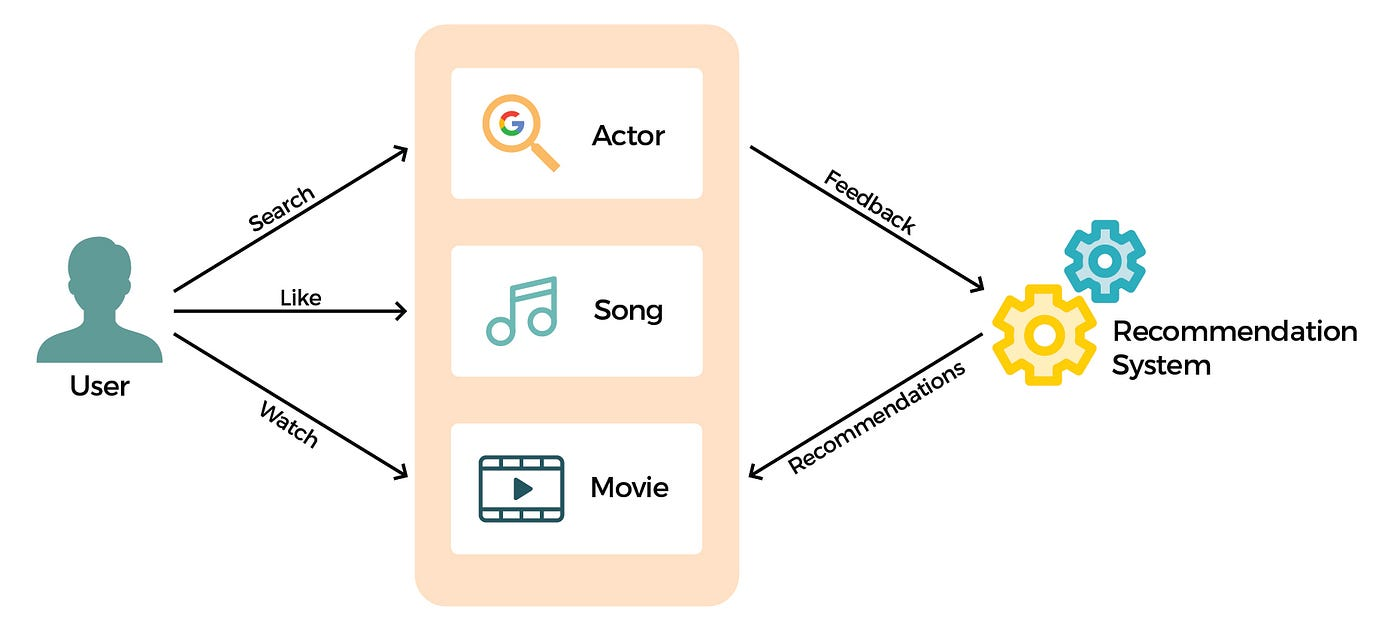
\includegraphics[height=0.4\textheight]{../documentazione/img/RecSys.png}
    \caption{Example of a Recommender System}
  \end{figure}
\end{frame}


\begin{frame}{Multimodal Recommender Systems}
  \begin{itemize}
    \item Use multiple modalities (text, image, audio) to enrich item representations \cite{Spillong}
    \item Encoding options: concat, fusion/attention, GNNs \cite{ConcatFeature, Fusion}
  \end{itemize}
  \begin{figure}[h]
    \centering
    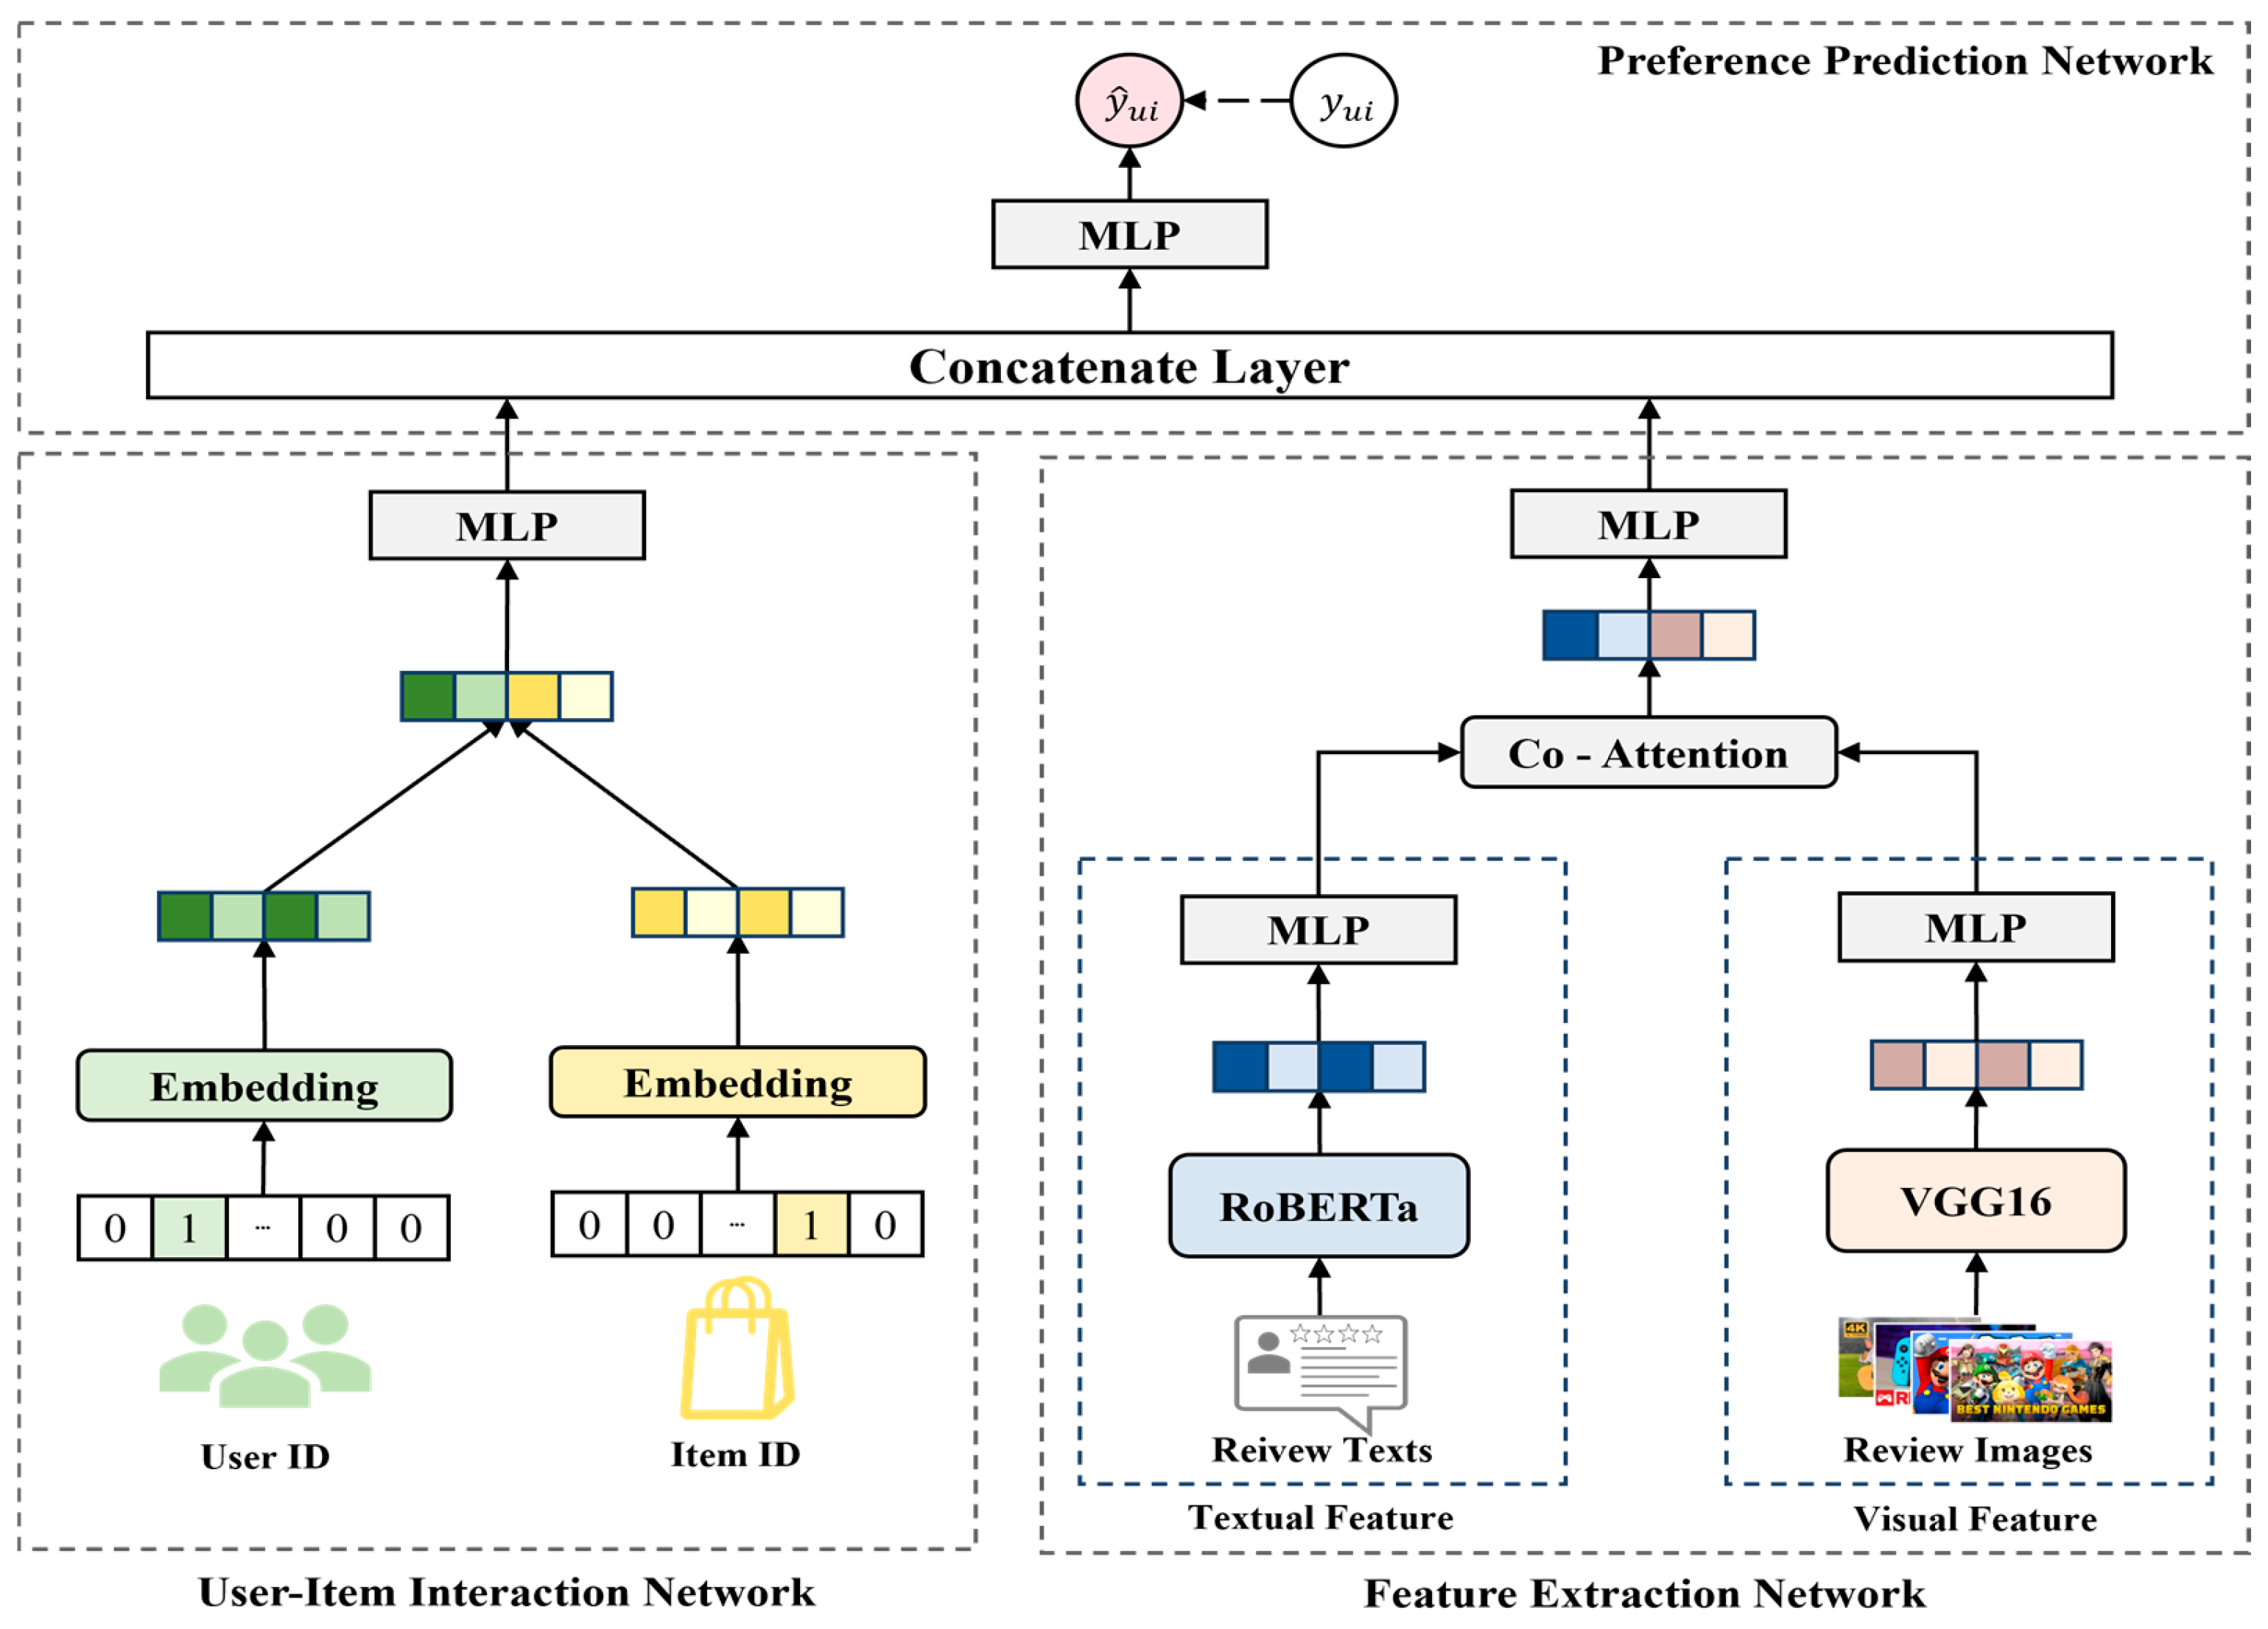
\includegraphics[height=0.4\textheight]{../documentazione/img/MMRec.png}
    \caption{Example of a Multimodal Recommender System}
  \end{figure}
\end{frame}

%\begin{frame}{MMRec Dataset extensions}
  %\begin{itemize}
  %  \item Multimodal extensions for MovieLens-1M and LastFM: additional text, images, audio and video were collected and encoded to create aligned and disaligned feature sets \cite{Spillong}
  %  \item These datasets enable full multimodal benchmarking and allow to assess the impact of alignment across domains
  %\end{itemize}
%\end{frame}

% ------------------------- Aligned Models -------------------------
\section{Aligned Models}
\begin{frame}{Contrastive Learning}
  \begin{itemize}
    \item Self-supervised method learning representations that bring similar samples closer \cite{ContrastiveLearning}
    \item Contrastive loss: $\ell_{i,j} = -\log \frac{\exp(\text{sim}(z_i, z_j)/\tau)}{\sum_{k=1}^{2N} [k \neq i] \exp(\text{sim}(z_i, z_k)/\tau)}$
  \end{itemize}
  \begin{figure}[h]
    \centering
    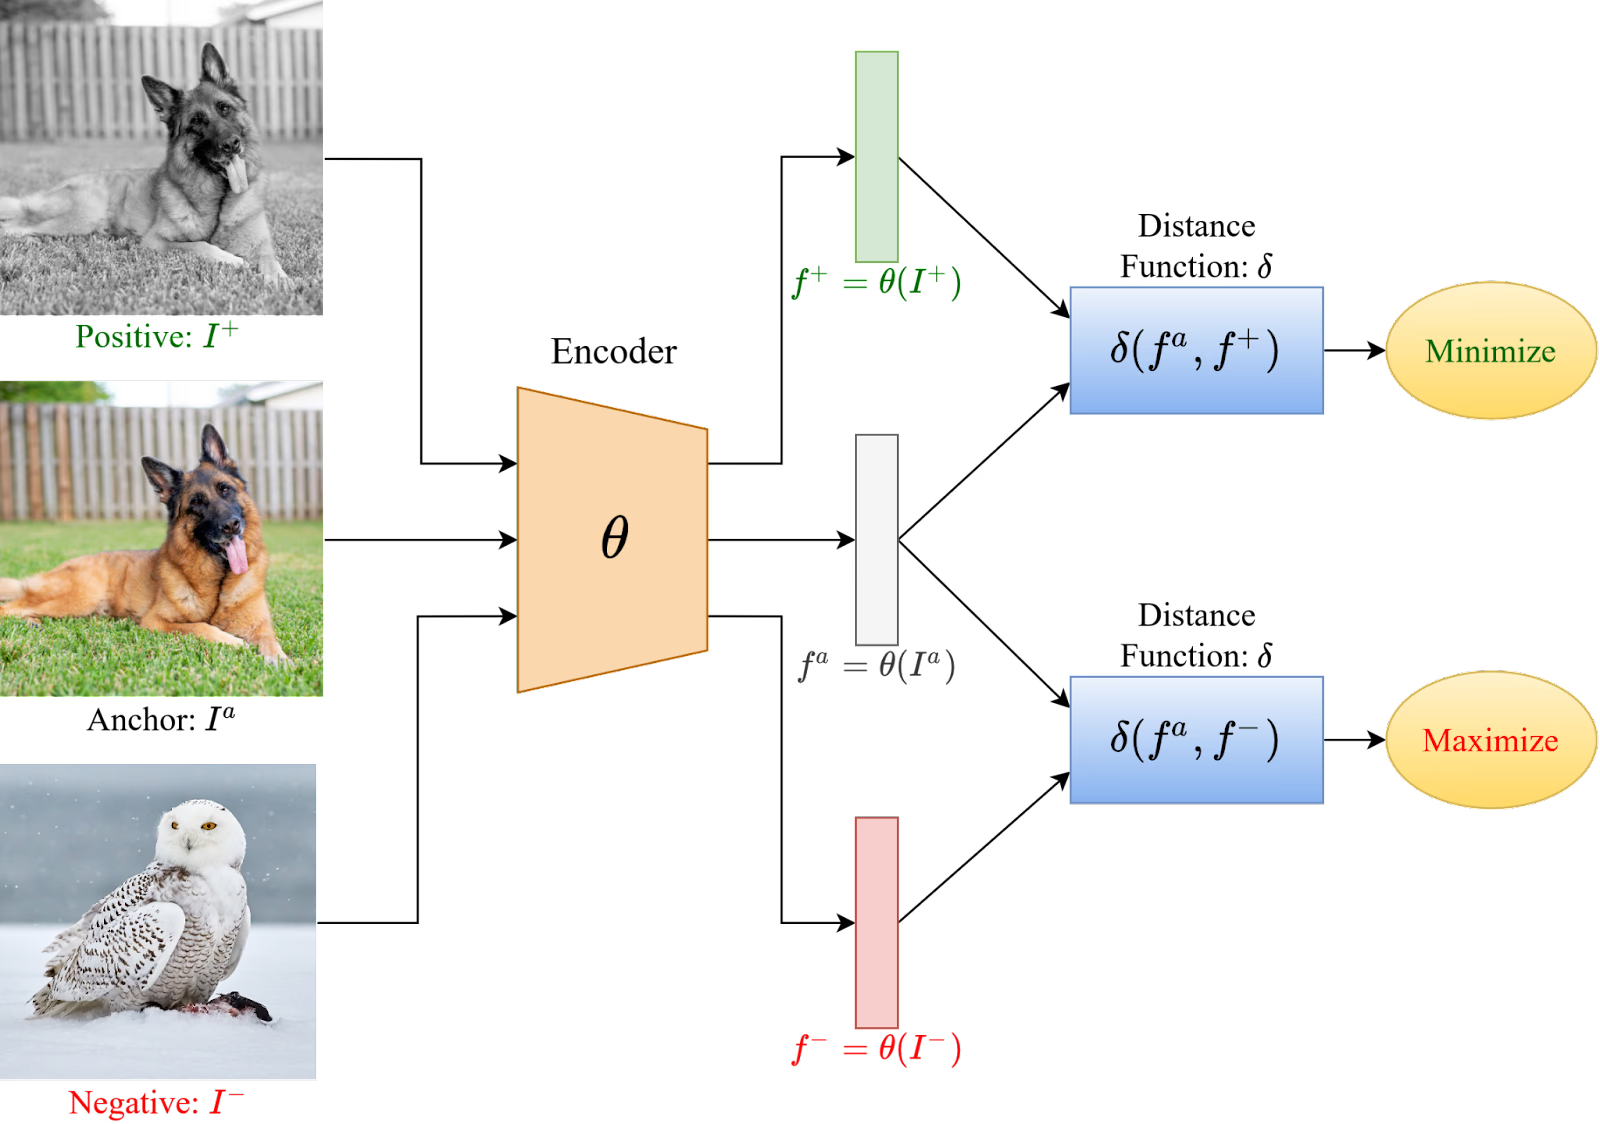
\includegraphics[width=0.4\textwidth]{../documentazione/img/CLearning.png}
    \caption{Conceptual representation of Contrastive Learning}
  \end{figure}
\end{frame}

\begin{frame}{CLIP}
  \begin{itemize}
    \item CLIP aligns image and text embeddings in a shared space (OpenAI) \cite{CLIP}
    \item Recent work shows that large multimodal encoders like CLIP can effectively improve recommender system performance when fine-tuned appropriately \cite{CLIPRecSys}
  \end{itemize}
  \begin{figure}[h]
    \centering
    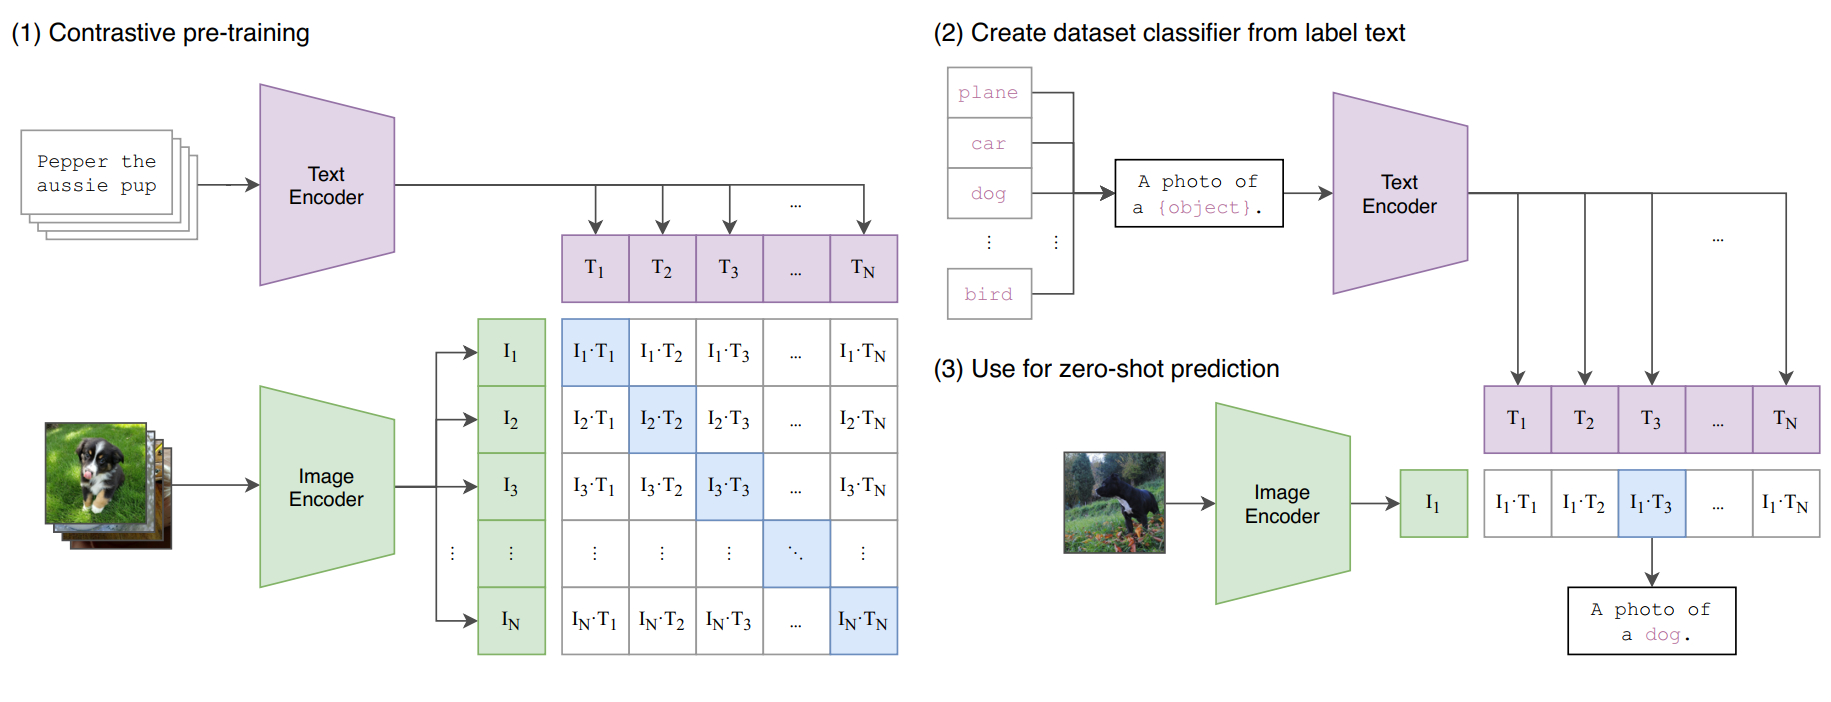
\includegraphics[height=0.4\textheight]{../documentazione/img/CLIP.png}
    \caption{Conceptual representation of CLIP architecture}
  \end{figure}
\end{frame}

\begin{frame}{AudioCLIP}
  \begin{itemize}
    \item Extends CLIP by adding an audio encoder (ESResNeXt) to the tri-modal alignment \cite{AudioCLIP}
    \item Training: audio-head pretrain, cooperative distillation, full tri-modal fine-tuning on AudioSet
  \end{itemize}
  \begin{figure}[h]
    \centering
    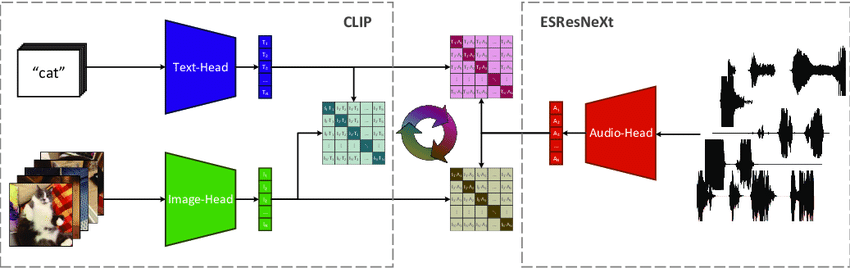
\includegraphics[height=0.3\textheight]{../documentazione/img/AudioCLIP.png}
    \caption{Conceptual representation of AudioCLIP architecture}
  \end{figure}
\end{frame}

% ------------------------- Experimental Settings -------------------------
\section{Experimental Settings}
\begin{frame}{Research Questions, Datasets and Models}
  \textbf{RQ1:} Can aligned multimodal embeddings improve recommender performance?
  Considered dataset:
  \begin{itemize}
    \item MovieLens 1M: movies with posters, trailers (audio), and text descriptions
    \item LastFM: artist-level interactions, track-level multimodal features (images, audio, text)
  \end{itemize}

  Considered models:
  \begin{itemize}
    \item BPR: Bayesian Personalized Ranking
    \item VBPR: extension of BPR incorporating for multimodal recommendation
    \item LATTICE: GNN-based model for multimodal recommendation (with 1 or 3 layers)
    \item FREEDOM: GNN-based model with modality-specific encoders and attention-based fusion (3 layers)
  \end{itemize}

\end{frame}
%
%\begin{frame}{Embedding Extraction Pipeline}
 % \begin{enumerate}
  %  \item File discovery and strict alignment across modalities
   % \item Extraction using both aligned (CLIP, AudioCLIP) and modality-specific (ViT, MiniLM, VGGish) encoders
    %\item 5-core filtering and ID remapping
  %\end{enumerate}
%\end{frame}
%
% ------------------------- Experiments -------------------------
\section{Experiments}
\begin{frame}{Embedding distribution technique}
  \begin{itemize}
    \item UMAP (Uniform Manifold Approximation and Projection) is used to reduce high-dimensional embeddings to 2D preserving local/global structure.
    \item After UMAP, we center and S1-normalize points: $\mathbf{x}_i' = \mathbf{x}_i - \bar{\mathbf{x}}$, $\mathbf{x}_i'' = \frac{\mathbf{x}_i'}{\|\mathbf{x}_i'\|}$.
    \item Spatial density: 2D Gaussian Kernel Density Estimation (KDE) on the projected points.
  \end{itemize}
\end{frame}
\begin{frame}{MovieLens 1M: CLIP-aligned Text+Image}
  \begin{figure}[h]
    \centering
    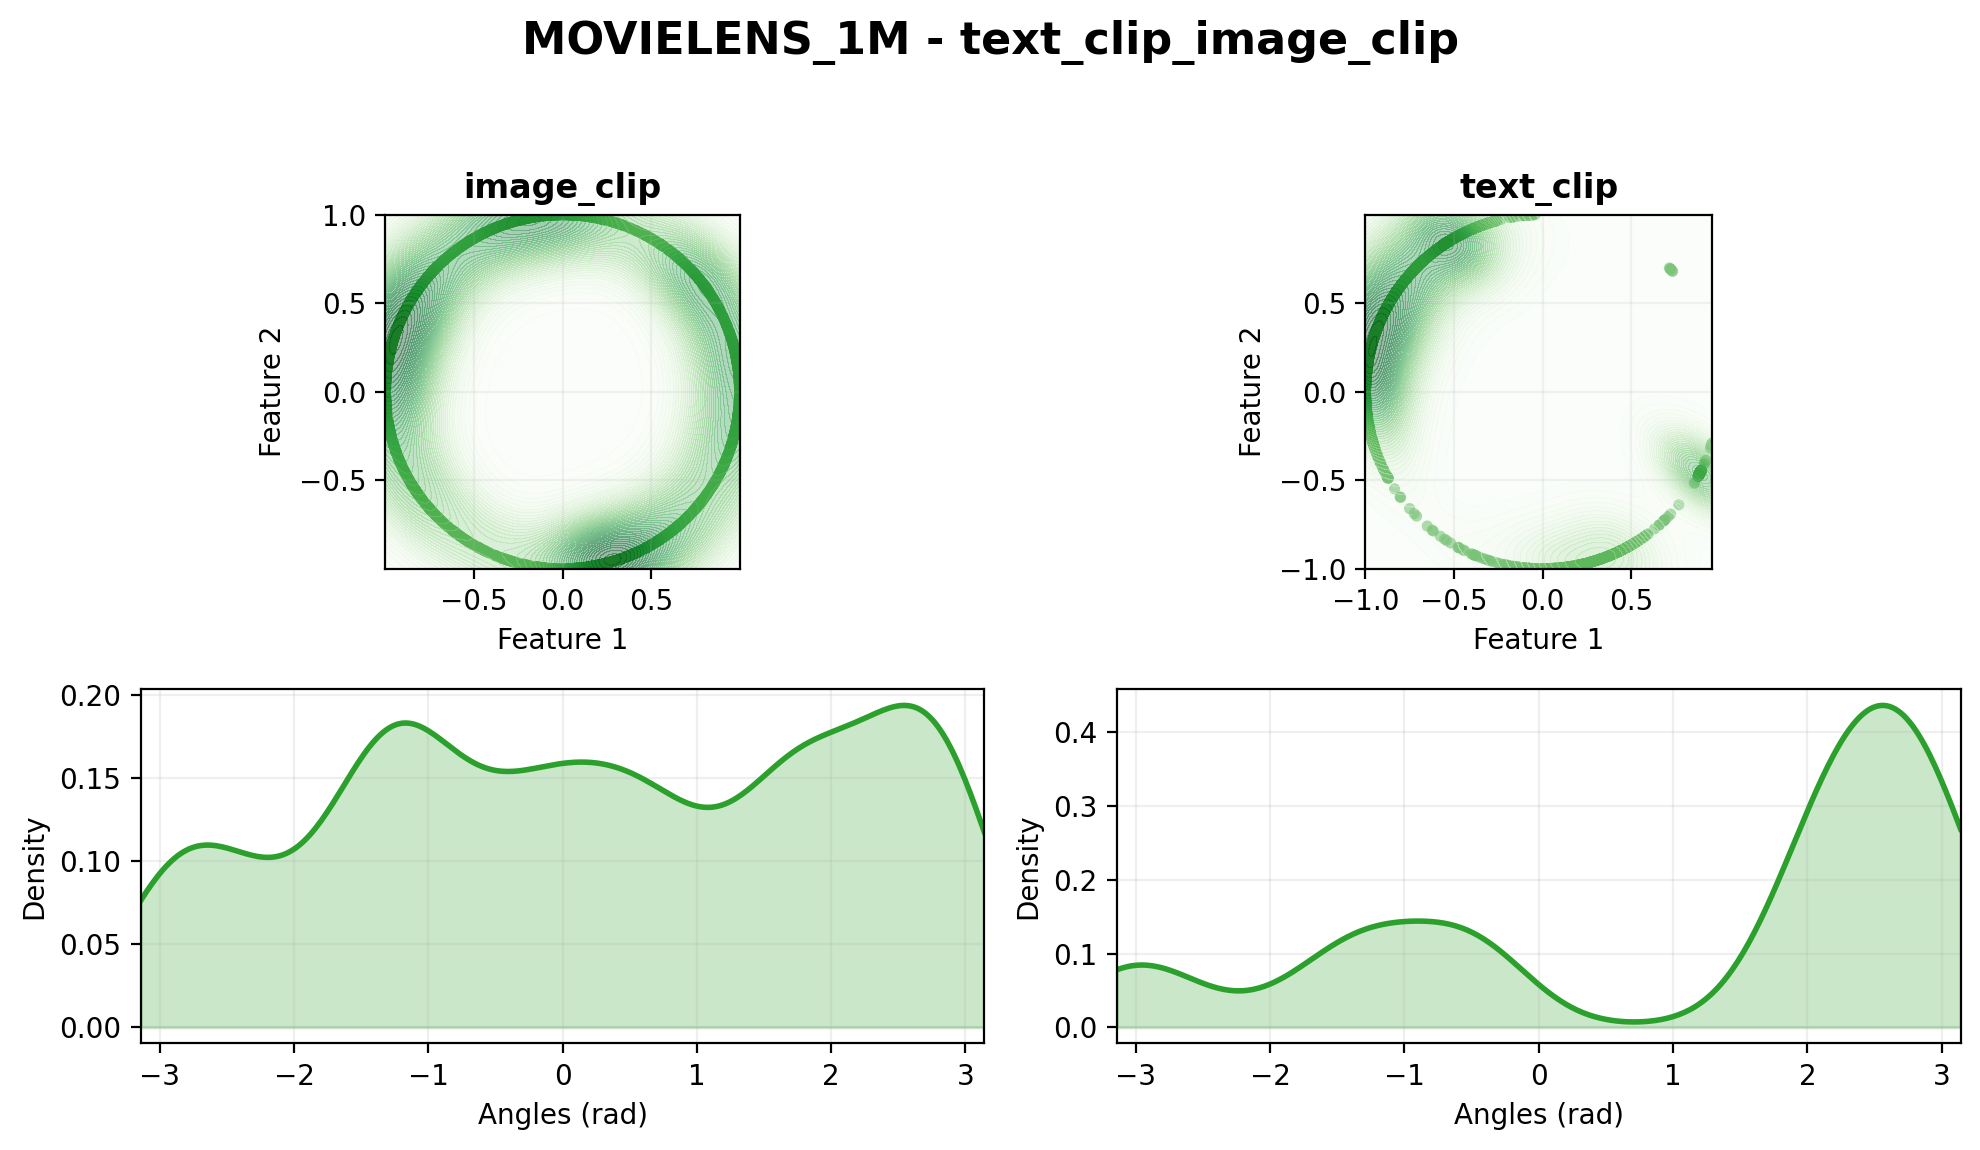
\includegraphics[width=0.95\textwidth]{../data/reports/experiment_plots/movielens_1m_LATTICE_text_clip_image_clip_kde.png}
    \vspace{2mm}
  \end{figure}
\end{frame}

\begin{frame}{MovieLens 1M: AudioCLIP aligned (Text+Image+Audio)}
  \begin{figure}[h]
    \centering
    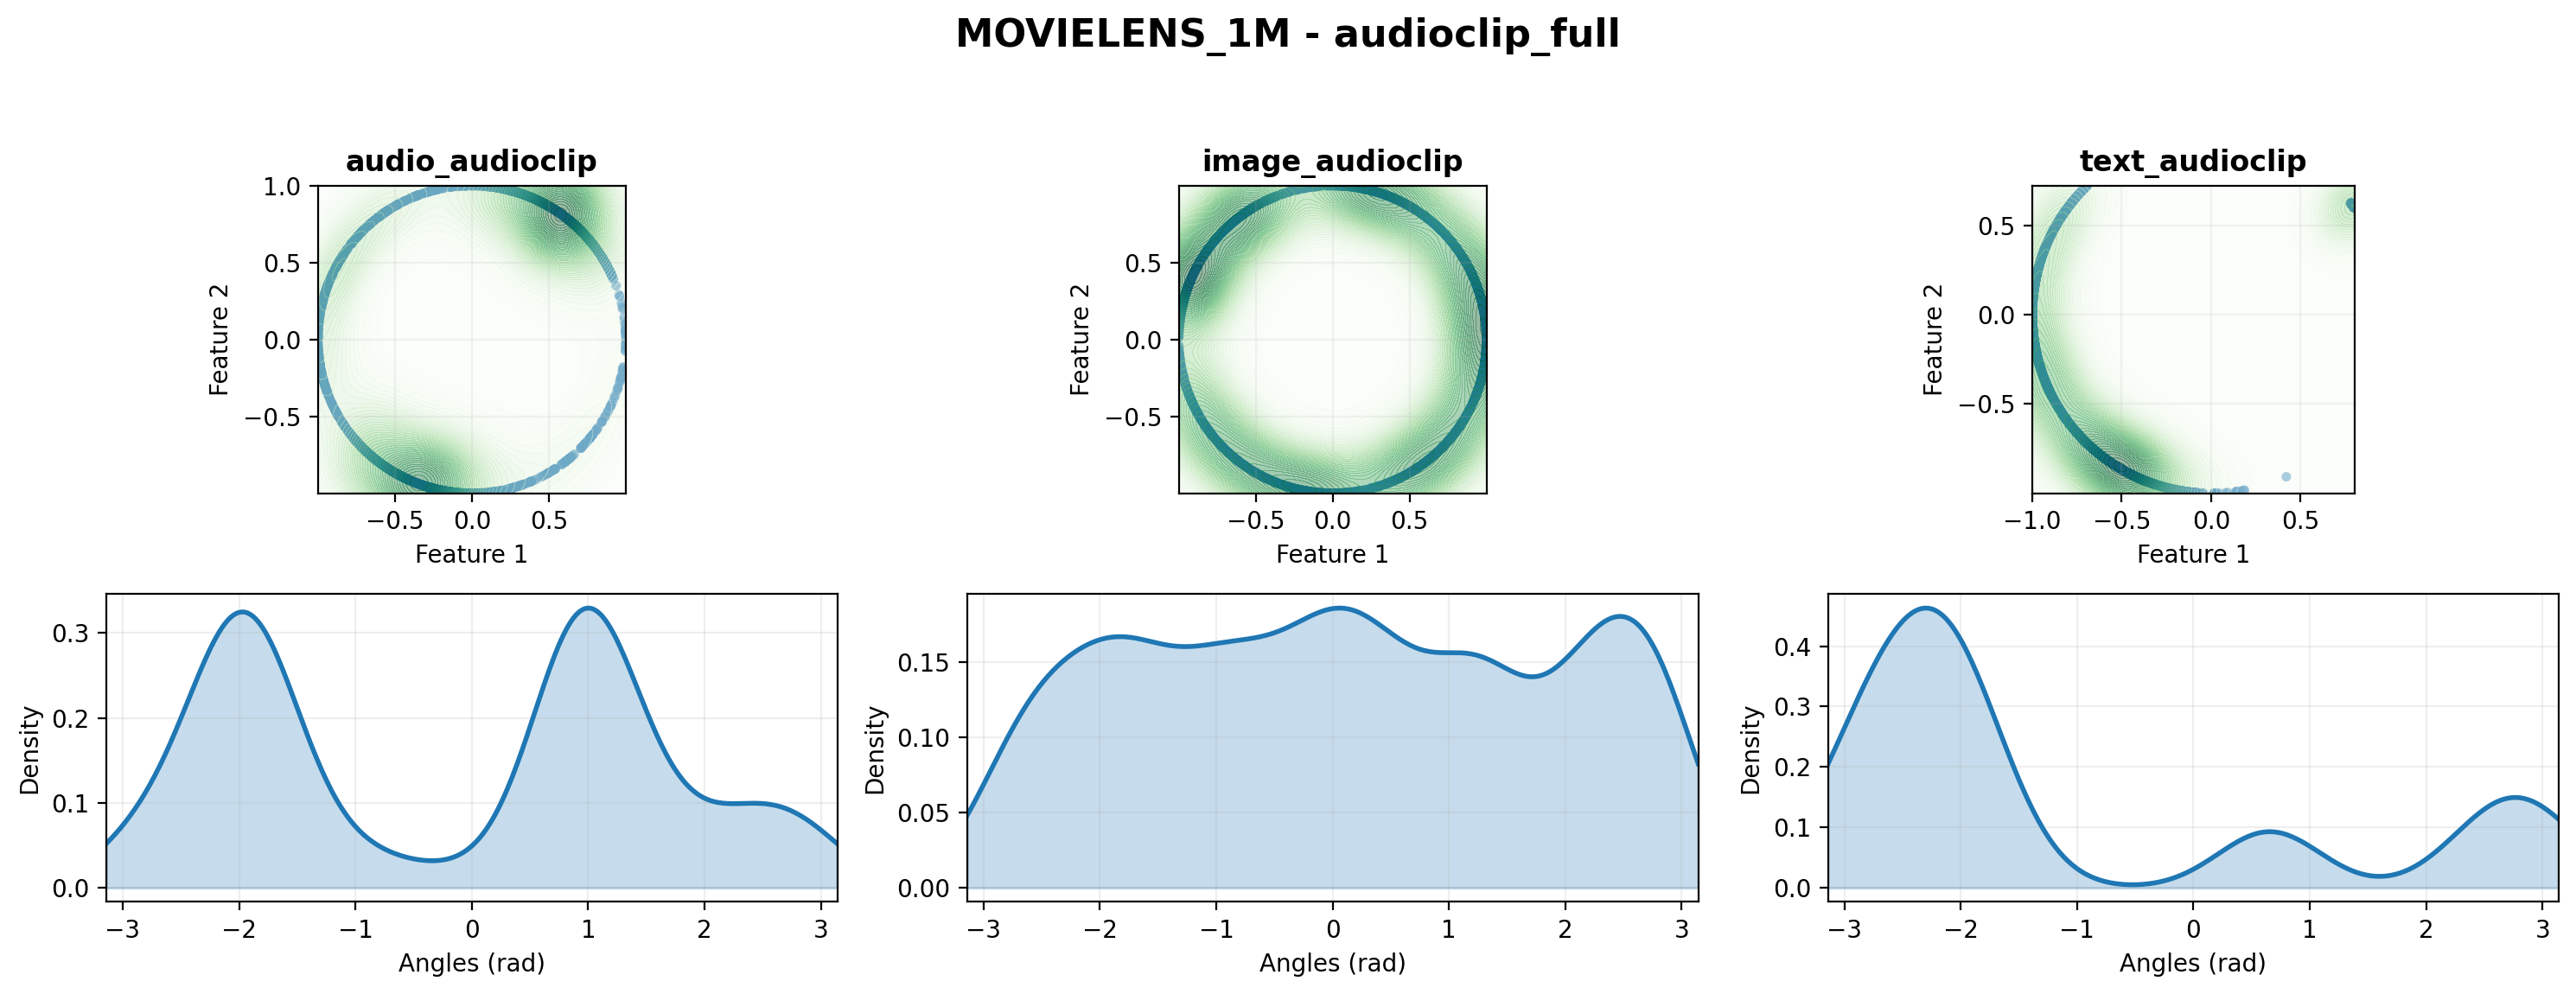
\includegraphics[width=0.95\textwidth]{../data/reports/experiment_plots/movielens_1m_LATTICE_audioclip_full_kde.png}
    \vspace{2mm}
   
  \end{figure}
\end{frame}

\begin{frame}{MovieLens 1M: Disaligned Text+Image+Audio (MiniLM+ViT+VGGish)}
  \begin{figure}[h]
    \centering
    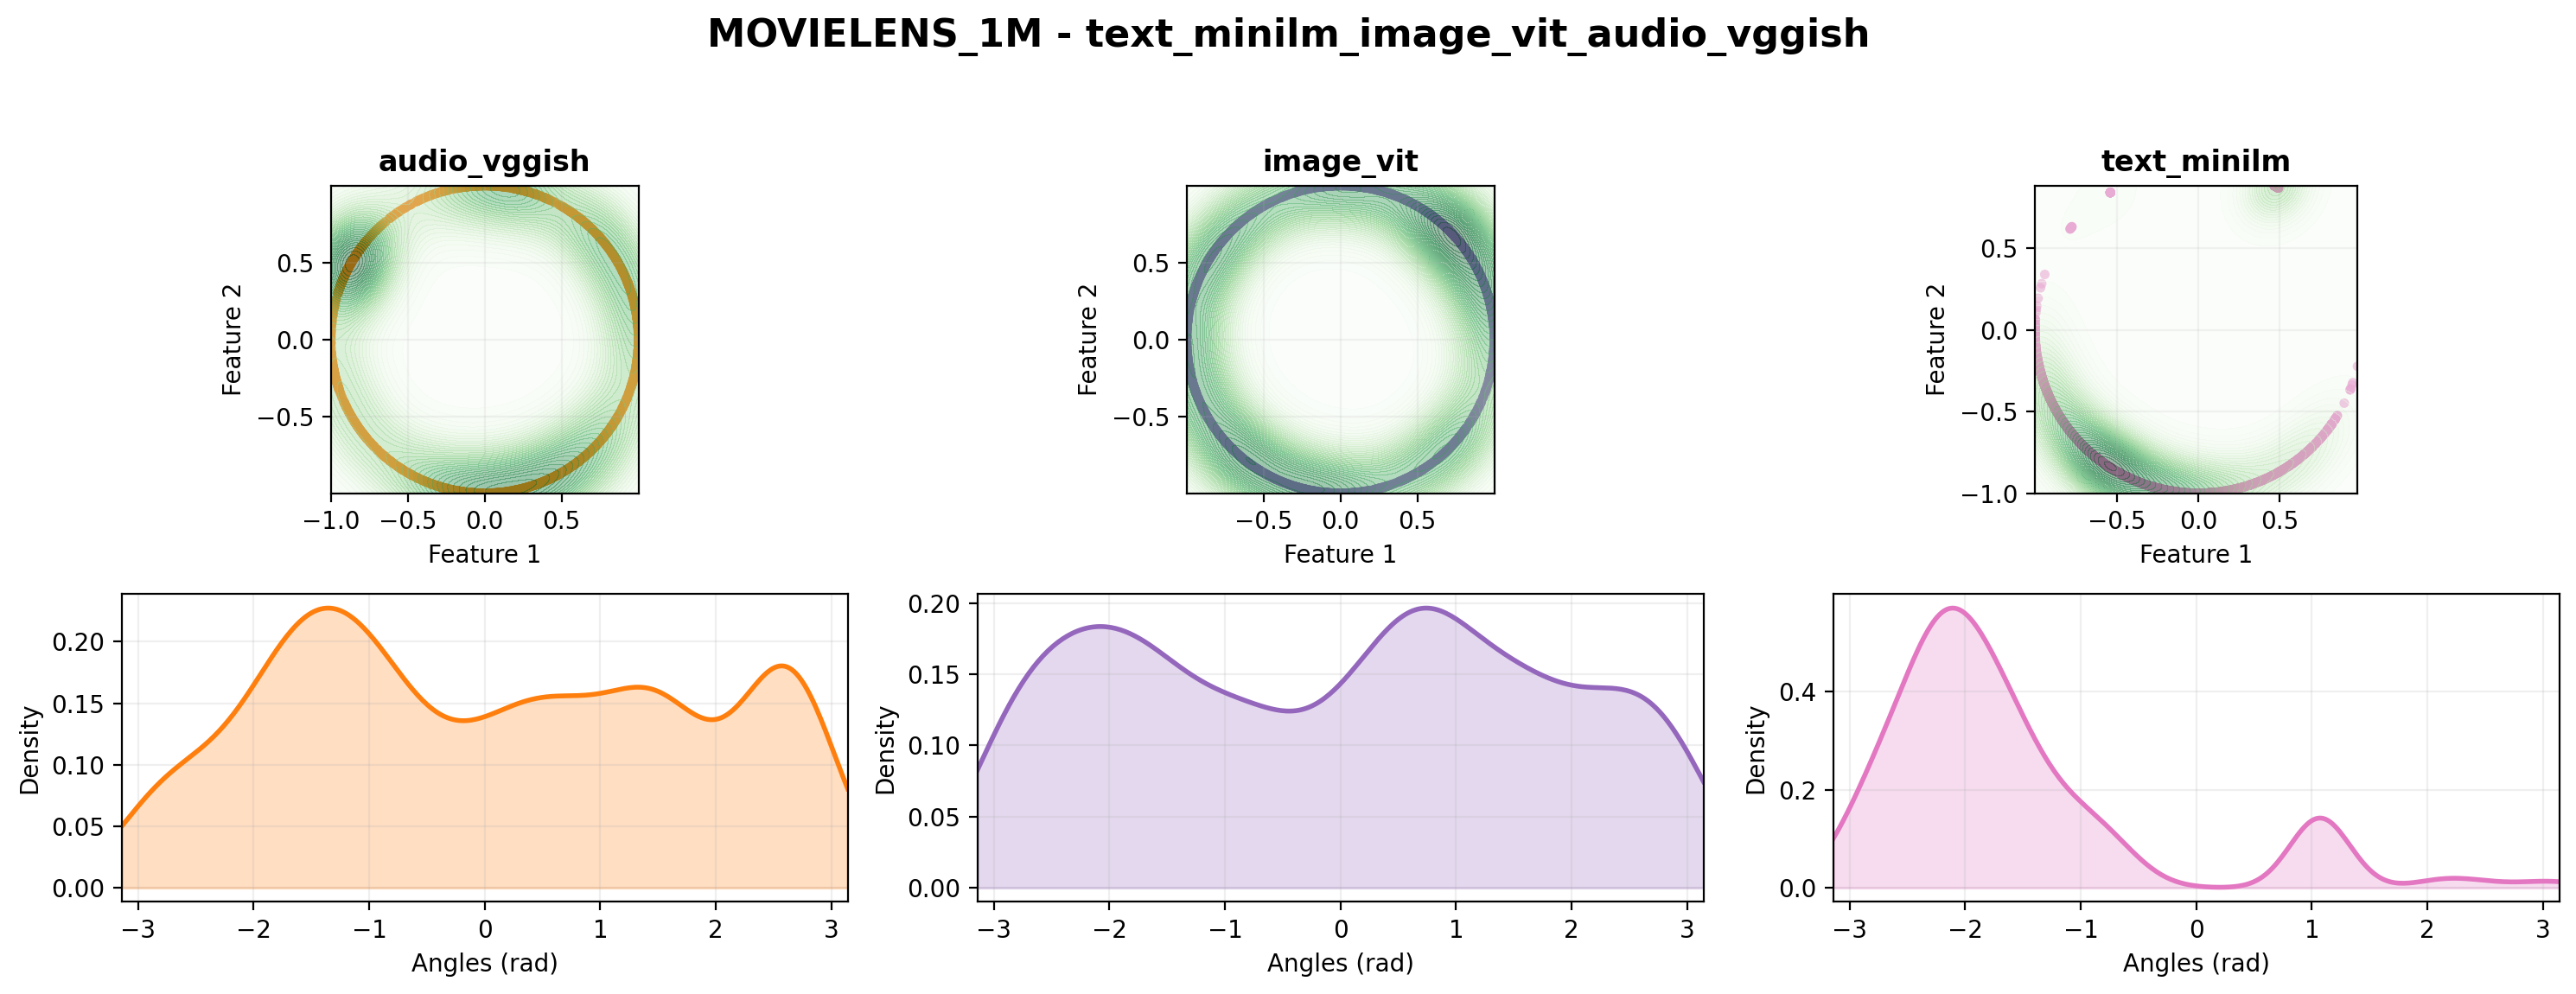
\includegraphics[width=0.95\textwidth]{../data/reports/experiment_plots/movielens_1m_LATTICE_text_minilm_image_vit_audio_vggish_kde.png}
    \vspace{2mm}

  \end{figure}
\end{frame}


\begin{frame}{Quantitative comparison: MovieLens (k=5)}
  \begin{table}[h]
    \centering
    \resizebox{\textwidth}{!}{
    \begin{tabular}{lcccc}
    	\toprule
    Model & Rec@5 & NDCG@5 & Prec@5 & MAP@5 \\
    \midrule
    BPR & 0.1089 & 0.2096 & 0.1898 & 0.1289 \\
    VBPR (CLIP) & 0.1152 & \textbf{0.2205} & \textbf{0.1997} & \textbf{0.1376} \\
    VBPR (AudioCLIP) & 0.0940 & 0.1857 & 0.1694 & 0.1125 \\
    VBPR (Disaligned) & 0.1163 & 0.2191 & 0.1986 & 0.1356 \\
    LATTICE\_3 (CLIP) & 0.1134 & 0.2189 & 0.1977 & 0.1359 \\
    LATTICE\_3 (AudioCLIP) & 0.1120 & 0.2183 & 0.1988 & 0.1358 \\
    LATTICE\_3 (Disaligned) & 0.1132 & 0.2179 & 0.1971 & 0.1349 \\
    FREEDOM (CLIP) & 0.1106 & 0.2150 & 0.1930 & 0.1331 \\
    FREEDOM (AudioCLIP) & \textbf{0.1164} & 0.2204 & 0.1984 & 0.1373 \\
    FREEDOM (Disaligned) & 0.1106 & 0.2158 & 0.1938 & 0.1337 \\
    \bottomrule
    \end{tabular}
    }
    \caption{MovieLens 1M - Comparison at cutoff k=5}
  \end{table}
\end{frame}

\begin{frame}{Quantitative comparison: MovieLens (k=10)}
  \begin{table}[h]
    \centering
    \resizebox{\textwidth}{!}{
    \begin{tabular}{lcccc}
    	\toprule
    Model & Rec@10 & NDCG@10 & Prec@10 & MAP@10 \\
    \midrule
    BPR & 0.1776 & 0.2159 & 0.1631 & 0.1120 \\
    VBPR (CLIP) & \textbf{0.1911} & \textbf{0.2300} & \textbf{0.1745} & \textbf{0.1211} \\
    VBPR (AudioCLIP) & 0.1570 & 0.1922 & 0.1476 & 0.0969 \\
    VBPR (Disaligned) & 0.1876 & 0.2271 & 0.1718 & 0.1195 \\
    LATTICE\_3 (CLIP) & 0.1877 & 0.2275 & 0.1721 & 0.1198 \\
    LATTICE\_3 (AudioCLIP) & 0.1875 & 0.2266 & 0.1725 & 0.1188 \\
    LATTICE\_3 (Disaligned) & 0.1848 & 0.2257 & 0.1710 & 0.1183 \\
    FREEDOM (CLIP) & 0.1796 & 0.2211 & 0.1657 & 0.1158 \\
    FREEDOM (AudioCLIP) & 0.1844 & 0.2259 & 0.1688 & 0.1193 \\
    FREEDOM (Disaligned) & 0.1801 & 0.2215 & 0.1658 & 0.1161 \\
    \bottomrule
    \end{tabular}
    }
    \caption{MovieLens 1M - Comparison at cutoff k=10}
  \end{table}
\end{frame}

\begin{frame}{Quantitative comparison: LastFM (k=5)}
  \begin{table}[h]
    \centering
    \resizebox{\textwidth}{!}{
    \begin{tabular}{lcccc}
    	\toprule
    Model & Rec@5 & NDCG@5 & Prec@5 & MAP@5 \\
    \midrule
    BPR & 0.0655 & 0.1595 & 0.1577 & 0.1414 \\
    VBPR (CLIP) & 0.0707 & 0.1714 & 0.1691 & 0.1524 \\
    VBPR (AudioCLIP) & 0.0694 & 0.1735 & 0.1711 & 0.1531 \\
    VBPR (Disaligned) & \textbf{0.0768} & \textbf{0.1859} & \textbf{0.1831} & \textbf{0.1660} \\
    LATTICE\_3 (CLIP) & 0.0726 & 0.1762 & 0.1751 & 0.1564 \\
    LATTICE\_3 (AudioCLIP) & 0.0712 & 0.1742 & 0.1718 & 0.1538 \\
    LATTICE\_3 (Disaligned) & 0.0757 & 0.1856 & 0.1825 & 0.1646 \\
    FREEDOM (CLIP) & 0.0522 & 0.1357 & 0.1358 & 0.1303 \\
    FREEDOM (AudioCLIP) & 0.0526 & 0.1358 & 0.1358 & 0.1299 \\
    FREEDOM (Disaligned) & 0.0527 & 0.1362 & 0.1362 & 0.1306 \\
    \bottomrule
    \end{tabular}
    }
    \caption{LastFM - Comparison at cutoff k=5}
  \end{table}
\end{frame}

\begin{frame}{Quantitative comparison: LastFM (k=10)}
  \begin{table}[h]
    \centering
    \resizebox{\textwidth}{!}{
    \begin{tabular}{lcccc}
    	\toprule
    Model & Rec@10 & NDCG@10 & Prec@10 & MAP@10 \\
    \midrule
    BPR & 0.1132 & 0.1534 & 0.1404 & 0.1061 \\
    VBPR (CLIP) & 0.1222 & 0.1646 & 0.1488 & 0.1149 \\
    VBPR (AudioCLIP) & 0.1196 & 0.1636 & 0.1482 & 0.1136 \\
    VBPR (Disaligned) & \textbf{0.1307} & \textbf{0.1755} & \textbf{0.1560} & \textbf{0.1242} \\
    LATTICE\_3 (CLIP) & 0.1232 & 0.1667 & 0.1507 & 0.1160 \\
    LATTICE\_3 (AudioCLIP) & 0.1238 & 0.1669 & 0.1510 & 0.1160 \\
    LATTICE\_3 (Disaligned) & 0.1258 & 0.1722 & 0.1535 & 0.1209 \\
    FREEDOM (CLIP) & 0.0986 & 0.1320 & 0.1225 & 0.0953 \\
    FREEDOM (AudioCLIP) & 0.0989 & 0.1323 & 0.1227 & 0.0953 \\
    FREEDOM (Disaligned) & 0.0986 & 0.1322 & 0.1224 & 0.0954 \\
    \bottomrule
    \end{tabular}
    }
    \caption{LastFM - Comparison at cutoff k=10}
  \end{table}
\end{frame}




% ------------------------- Discussion & Conclusion -------------------------
\section{Discussion \& Conclusion}
\begin{frame}{Discussion}
  \begin{itemize}
    \item Alignment helps when modalities share strong semantic relationships (e.g., posters and descriptions)
    \item Aggressive alignment (AudioCLIP) can erase modality-specific signals leading to worse ranking
    \item Simpler models (VBPR) can outperform complex GNNs when features are well represented
  \end{itemize}
\end{frame}

\begin{frame}{Conclusions and Future Work}
  \begin{itemize}
    \item Use domain-adaptive fusion strategies to select aligned/disaligned features
    \item Explore softer alignment / regularization strategies for audio
    \item Investigate model-feature co-design (when to use GNNs vs. projection models)
  \end{itemize}
\end{frame}

\begin{frame}{Thank you!}
  \begin{center}
    Thank you for your attention! \twemoji{rocket}
  \end{center}
\end{frame}



\begin{frame}[allowframebreaks]{References}
  \bibliographystyle{plain}
  \bibliography{../documentazione/biblio}
\end{frame}

\end{document}
